\documentclass[11pt]{article}

\usepackage[top=1.5in, bottom=1.5in, left=1in, right=1in]{geometry}

\usepackage{algorithm}
\usepackage{mathtools}
\usepackage{algorithmic}
\usepackage{graphicx}
\usepackage{multirow}
\usepackage{float}
\usepackage{pdfpages}
\usepackage{listings}
\usepackage{booktabs}

\PassOptionsToPackage{hyphens}{url}\usepackage{hyperref}
\author{Matthew Smith}
\title{CS909: Exercise 8 Report}
\date{\today}

\begin{document}
\maketitle

\section{Introduction}
This report describes the design, implementation and evaluation of a range of feature sets, classifiers and clustering algorithms whilst working with a large body of text data. The system was implemented in Python and used a range of packages to aid development. Whilst they will be named in the relevant sections, the packages used were:
\begin{itemize}
\item Natural Language Processing Toolkit (NLTK)~\cite{nltk}
\item GenSim~\cite{gensim}
\item Scikit-Learn (SKLearn)~\cite{scikit-learn}
\item Beautiful Soup 4~\cite{bs4}
\item LXML~\cite{lxml}
\end{itemize}

The code for this project can be found at \url{https://github.com/tangohead/CS909-Project}.
\section{Pre-processing and Data Description}
\label{preproc}
The data took the form of a large set of XML-encoded Reuters news articles from the year of 1987, known as \emph{Reuters-21578}.  It contains 21578 articles, each labelled with a range of attributes. Important elements for each article with respect to this project were:
\begin{itemize}
\item \texttt{LEWISSPLIT} – identifying whether the article was in the train or test sets, or neither
\item \texttt{TOPICS} – the list of topics associated with this article
\item \texttt{BODY} – within the \texttt{TEXT} element group, this held the text of the story
\end{itemize}

The XML was parsed with \textit{Beautiful Soup 4} with the \textit{LXML} parser, which enabled quick and easy access to all sections of the document within Python. A range of elements were omitted, such as \texttt{TITLE}, \texttt{PLACES}, \texttt{DATELINE} and so on. Since the project specification did not require classification on these elements, omitting them at load-time saved memory and processing resources, which would be extremely important later in the execution. It was important to note that articles without topics, or with their \texttt{LEWISSPLIT} attribute as \texttt{NOT\_USED} were not loaded into the system. The former is to avoid attempting to train a classifier on an article with not label, and the latter is to adhere to the Lewis train/test split. Furthermore, only a subset of possible topics were used – these topics were: \textit{earn}, \textit{acq}, \textit{money-fx}, \textit{grain}, \textit{crude}, \textit{trade}, \textit{interest}, \textit{ship}, \textit{wheat} and \textit{corn}. For a given article, all tokens in this list were recorded, and any articles only assigned to topics outside of this list were not used. If an article contained some listed and some unlisted topics, only those listed were stored.

Pre-processing took the form of two main stages: tokenisation/trimming and language-based operations. The first of these took the body-text of an article and first removed a range of punctuation (+,/,\textless\textgreater,(),',",-) and date numbers (e.g. 1st), replacing it with a space. This was initially included to help with cases such as
\begin{itemize}
\item 1987/88, or
\item Red-yellow
\end{itemize}
In the first of these, not performing this step before tokenisation resulted a number that could not be directly parsed but instead had to be re-tokenised. In order to avoid passing over the entire article again after separating out the `1987/88', replacing the slash with a space avoided this. The second instance could either be merged into one word or split into two. To avoid having many, very specific tokens, the system instead opts to split them apart. Generally speaking, this step makes some assumptions about the structure of the sentences and where spaces can be inserted, but significantly reduces the number of possible tokens or extra computation required for re-tokenisation.


The articles were then tokenised using the NLTK tokeniser, which produced the basic bag of words. A number of steps were performed. Each token had:
\begin{enumerate}
\item Commas or full-stops removed without replacement. This is specifically to account for acronyms, which should not be space-separated as they will lose their meaning. It does, however, act on numbers as well, but these are removed in a later step.
\item Check if the token is `Reuters' – this word is common as a final line in the article, without context. Removing this avoids artificially representing it
\item Checking for and removing the token if it is a stop word, according to NLTK’s stop word list, removing items such as `the', or `am', which do not add to classification and only act to bulk out the bag of words.
\item Removing numbers, as again these are usually too specific (e.g. stock prices) or too general (e.g. year) to be useful in classification.
\end{enumerate}

The word set at this point has been significantly reduced and should represent the core themes of the article through the remaining words in the article. This aids in avoiding unrepresentative terms (such as stop words or numbers) skewing the features or classification, and makes the data easier to fit in memory. This section can be seen in the \texttt{trim\_and\_token} method of \texttt{helper.py}.

Secondly, language processing helps contextualise the set of words generated in the previous step. This again involved a number of steps:
\begin{enumerate}
\item The tokens were \textit{part-of-speech} (POS) tagged to indicate which linguistic category each belonged in. This was found to be particularly intensive and formed a large part of the runtime in later tests.
\item Using the POS tags, NLTK's \textit{Named Entity} (NE) recongiser ran over the tokens to indicate any NEs present. Each NE was then combined into a single token by underscores to flatten the data structure and make classification easier. For example, `British Airways Plc' would be converted to `British\_Airways\_Plc'.
\item If the token is not part of an NE, it is stemmed using NLTK's stemming algorithm. This helps reduce the number of variants on a word to the core of a word. Ideally, this will further condense the article content down to the themes, but ultimately helps in classfication as two forms of the same word will be able to be treated as one.
\end{enumerate}

At this point, the articles are represented as a condensed, tokenised form of the original. The overall aim of this step was to reduce the data such that as much non-topic-specific content is removed as possible, whilst avoiding causing overfitting by being excessive on the trimming. This part of the processing can be seen in the \texttt{lang\_proc} method of \texttt{helper.py}.

\section{Feature Representation}
Two groups of feature sets were tested in this project. One consisted of \textit{ngrams} alone, the other of \textit{ngram-based topic models}. All ngrams computed were preprocessed in the way described in section~\ref{preproc}. Whilst this does eliminate some of the structure imposed in bi- or trigrams, it serves to reduce the size of the documents and rid it of data which would not contribute to classification. Furthermore, the pre-processing provided a unigram representation as output, which was the base of all features produced in this section.

Within ngrams, three types were used: \textit{unigrams}, \textit{bigrams} and \textit{trigrams}. In general, ngrams were used since they provide a strong baseline – they directly represent the article content, are easy to manipulate and relatively quick to compute compared to something such as verbs or grammatical features. It should be noted that these features would also rely on the accuracy of the tagger used to identify them, so instead using ngrams avoids having to deal with this. Three types of ngram were used to experiment with incorporating sentence structure into the article representation: unigrams (i.e. bag of words) were used to provide a structure-free representation, whilst bigrams and trigrams were used to incorporate structure to some extent. Both bigrams and trigrams were generated by passing over the pre-processed dataset and combining and joining $n$ consecutive tokens with underscores, where $n=2$ for bigrams and $n=3$ for trigrams. Using all three provided a direct comparison over the incorporation of structure into document representation. Ngram generation can be seen in the \texttt{gen\_ngrams} method of \texttt{helper.py}.

Topic models were used as an alternative method to direct representation. The method used was to generate a topic model for each document which could then be used for classification - topic models were created based on the generator trained on the entire corpus. Although topic models are usually used in a fashion similar to clustering algorithms, here they were used to generate features. To investigate the effects of incorporating sentence structure on topic models, uni-, bi- and trigrams were used to train and generate features. In terms of implementation, the topic modelling package GenSim handled the training and creation of the features. It was trained with a corpus constructed from the entire training set and told to estimate for 10 topics, in order to match the number of topics being used for classification. The Latent Dirichlet allocation~\cite{lda} method was used to do this. The \texttt{gen\_topic\_model} and \texttt{gen\_topic\_model\_ngram} methods of \texttt{helper.py} implement this section.

It should be noted that the same generation technique was used for bigrams and trigrams that were used `raw' to classify articles, and that were fed into the topic models. A key difference, however, is that the `raw' token classification had to filter the bi- and trigrams to only use those which appear at least 10 times over all articles, whereas topic models did not filter this at all. This was because when attempting to classify the data, a vector space model of each document had to be built. 

To do this, an $n$ length vector had to be created, with each element representing a single bi- or trigram. Creating these ngrams results in many rare combinations which appear very few times across the corpus – these hardly contribute to classification and mainly serve to extend the size of the vector space. As described later, each document had to be vectorised before classification, and if these rare ngrams were not trimmed, the resulting training vector became extremely large and often expended memory supply. Whilst applying a frequency threshold of 10 could trim out features that contribute in minor ways to classification, not doing this made the task extremely hard to compute. Topic models did not receive this filtering as each document was pre-processed into a topic model representation before the classification stage, significantly reducing the representation size of each document to the 10 predicted topics. Vectorisation can be seen in the \texttt{get\_bow\_vect\_data} method of \texttt{helper.py}.

\section{Classification Methods}

Three classifiers were tested in this project – a decision tree, naïve Bayes and random forests. Each was implemented using the Scikit-learn package. The three provide a variety of approaches – one tree based, one directly using probabilities and one using ensemble methods (specifically boosting).

In order to use the data with the SKLearn classifiers, it first had to be transformed into a vector space model. This involves producing an n length vector, each element of which represents a type of feature that occurs across the entire data set. Using this, each document can be expressed in terms of a vector – at the most basic level, a binary count, any term that occurs in a document is recorded with a one in its corresponding element. This system required a slightly more complex approach in order to handle the size of the dataset. Term Frequency-Inverse Document Frequency (TF-IDF), seen in Equation~\ref{tfidf} which instead provides a gauge of how representative a particular term is of the document.  To calculate the TF-IDF of a term, the normalised Term Frequency (Equation~\ref{tf}) must be calculated, which can be biased to more unusual words. This is followed by the Inverse Document Frequency, seen in Equation~\ref{idf} with $df(t, D)$ being defined in~\ref{df} where $D$ is the set of documents. To produce the document vectors, a \texttt{tfidfVectorizer} and dictionary were created with the corpus then used to produce a vector for each document.

\begin{equation}
\label{tfidf}
TF-IDF = tf \times idf
\end{equation}

\begin{equation}
\label{tf}
tf(t,d) = \frac{\text{frequency of term } t \text{ in document d}}{\text{max. frequency of } t \text{ in any document d}}
\end{equation}
\begin{equation}
\label{idf}
idf(t,D) = \log\frac{\left\vert{D}\right\vert}{df(t, D)}
\end{equation}
\begin{equation}
\label{df}
df(t,D) = \left\vert\{d \in D: t \in d\}\right\vert
\end{equation}


Some articles had multiple labelled topics in the dataset. To account for this in classification, the article was included as a separate instance for each topic. Whilst this could result in overfitting to certain instances, or bias due to overrepresentation, it was a better approach than just taking the first recorded topic. Doing that would lose a great deal of topics and potentially underrepresent certain classes if the topics are ordered.

Scikit-learn's decision tree is a form of the Classification and Regression Tests (CART)~\cite{trees}, itself close to C4.5~\cite{c45}. A tree method provides a clear and efficient model to train and test on. Importantly, this tree uses Gini impurity as a split criterion – through this, the inherent bias and preference for short trees of Information Gain is not a factor. The decision tree implementation can be seen in \texttt{build\_run\_DecTree} and \texttt{build\_topmod\_DecTree} in \texttt{helper.py}.


Na{\"i}ve Bayes offered a simple yet effective approach to text classification, specifically a Gaussian Na{\"i}ve Bayes~\cite{nb}. This makes the assumption that the likelihood of features is Gaussian, and calculates probabilities as in equation~\ref{naive}.  Although it takes a simple approach to classifying items, this fits well with the method taken in representing documents – they have been stripped down to basic forms. Since a range of features were being tested, having na{\"i}ve Bayes as a baseline provided a useful comparison point for the other classifiers, which take more sophisticated approached. No parameters are required for the na{\"i}ve Bayes model, emphasising the simplicity of it. This section is implemented in \texttt{build\_run\_NB} and \texttt{build\_topmod\_NB} in \texttt{helper.py}.

\begin{equation}
\label{naive}
P(x_{i} \vert y) = \frac{1}{\sqrt{2 \pi \sigma_{y}^{2}}}\exp\left(-\frac{(x_{i}-\mu_{y})^{2}}{2\pi \sigma_{y}^{2}}\right)
\end{equation}

The third model was a random forest~\cite{randomforests}. Since it is a bagging-type ensemble method, it has the advantage that it builds a range of classifiers over sub-samples of the data set in an effort to increase accuracy. It does this through having a range of better-than-average classifiers and averaging their output for test data. This helps to avoid having one classifier overfitting the data, which could happen on such a large dataset with so many features. As with the decision tree, the Gini impurity is used as a splitting criterion. By using this approach, the effectiveness of ensemble methods on this data could be judged with respect to the other classifiers. This can be see in \texttt{build\_run\_RF} and \texttt{build\_topmod\_RF} in \texttt{helper.py}.

All classifiers were tested with K-fold cross validation, for 10 rounds. This allowed testing over the training data for each classifier, producing comparison statistics such as recall, precision and accuracy without having to test on the same data that the classifier was trained upon. To do this, the \texttt{LEWISSPLIT} `train' set was used, then sampled over the 10 rounds by SKLearn K-fold~\cite{kf}. The implementation, including statistic calculation, can be seen in \texttt{run\_k\_fold} in \texttt{helper.py}.

\section{Results and Optimal Configuration Testing}
This section discusses the results of the tests from the both classifier and feature evaluation. Each combination was tested, meaning that a decision tree, naïve Bayes and random forest classifier was trained on each of:
\begin{itemize}
\item Unigrams (BOW)
\item Bigrams (BIG)
\item Trigrams (TRIG)
\item Unigram Topic Model (BOW-TM)
\item Bigram Topic Model (BIG-TM)
\item Trigram Topic Model (TRI-TM)
\end{itemize}

For each, classification accuracy, micro and macro precision and recall were calculated over the training set. Accuracy provides a useful indication of how likely a configuration is to correctly predict a topic. Precision indicates how likely the configuration is to `over-guess' and classify items as a topic even when they are – a score of one indicates that the system predicts the topics without making too many false guesses. Recall records how likely the system is to incorrectly guess a topic, where a recall of one indicates perfect classification. Within precision and recall, micro and macro averaged metrics can be used; these provide methods to average the statistics over multiple classes. Micro averaging works by taking the average using global true positive and true negative sums, whereas macro averaging uses a per-class sum of each, before taking the average. Tables~\ref{tab:acc},~\ref{tab:map},~\ref{tab:mar},~\ref{tab:mip} and~\ref{tab:mir} display these values for each classifier and feature set. Note that NB refers to na{\"i}ve Bayes, DT to decision tree and RF to random forests.

% Table generated by Excel2LaTeX from sheet 'Sheet5'
\begin{table}[htbp]
  \centering
  \caption{Feature and Classifier Accuracy}
    \begin{tabular}{r|rrrrrr}
    \toprule
          & BOW   & BIG   & TRI   & BOW-TM & BIG-TM & TRI-TM \\
    \midrule
    NB    & 0.7040 & 0.7943 & 0.7294 & 0.6421 & 0.4740 & 0.4244 \\
    DT    & 0.7922 & 0.7380 & 0.7226 & 0.6922 & 0.5654 & 0.5143 \\
    RF    & 0.7829 & 0.7700 & 0.7377 & 0.7492 & 0.6385 & 0.5754 \\
    \bottomrule
    \end{tabular}%
  \label{tab:acc}%
\end{table}%

\begin{table}[htbp]
  \centering
  \caption{Macro Averaged Precision}
    \begin{tabular}{r|rrrrrr}
    \toprule
          & BOW   & BIG   & TRI   & BOW-TM & BIG-TM & TRI-TM \\
    \midrule
    NB    & 0.5339 & 0.5948 & 0.4818 & 0.4368 & 0.2108 & 0.1605 \\
    DT    & 0.6144 & 0.4821 & 0.4627 & 0.4237 & 0.2649 & 0.2270 \\
    RF    & 0.6144 & 0.5881 & 0.5354 & 0.5079 & 0.3570 & 0.2845 \\
    \bottomrule
    \end{tabular}%
  \label{tab:map}%
\end{table}%

\begin{table}[htbp]
  \centering
  \caption{Macro Averaged Recall}
    \begin{tabular}{r|rrrrrr}
    \toprule
          & BOW   & BIG   & TRI   & BOW-TM & BIG-TM & TRI-TM \\
    \midrule
    NB    & 0.5370 & 0.5733 & 0.5266 & 0.4113 & 0.1841 & 0.1549 \\
    DT    & 0.5189 & 0.4838 & 0.4397 & 0.4448 & 0.2533 & 0.2398 \\
    RF    & 0.5189 & 0.5116 & 0.4676 & 0.4891 & 0.3273 & 0.2522 \\
    \bottomrule
    \end{tabular}%
  \label{tab:mar}%
\end{table}%

% Table generated by Excel2LaTeX from sheet 'Sheet5'
\begin{table}[htbp]
  \centering
  \caption{Micro Averaged Precision}
    \begin{tabular}{r|rrrrrr}
    \toprule
          & BOW   & BIG   & TRI   & BOW-TM & BIG-TM & TRI-TM \\
    \midrule
    NB    & 0.7040 & 0.7943 & 0.7294 & 0.6421 & 0.4739 & 0.4244 \\
    DT    & 0.7829 & 0.7380 & 0.7226 & 0.6922 & 0.5654 & 0.5143 \\
    RF    & 0.7829 & 0.7700 & 0.7377 & 0.7522 & 0.6385 & 0.5754 \\
    \bottomrule
    \end{tabular}%
  \label{tab:mip}%
\end{table}%

% Table generated by Excel2LaTeX from sheet 'Sheet5'
\begin{table}[htbp]
  \centering
  \caption{Micro Averaged Recall}
    \begin{tabular}{r|rrrrrr}
    \toprule
          & BOW   & BIG   & TRI   & BOW-TM & BIG-TM & TRI-TM \\
    \midrule
    NB    & 0.6769 & 0.7943 & 0.7294 & 0.6421 & 0.4740 & 0.4740 \\
    DT    & 0.7829 & 0.7380 & 0.7226 & 0.6949 & 0.5654 & 0.5654 \\
    RF    & 0.7829 & 0.7700 & 0.7377 & 0.7522 & 0.7522 & 0.6385 \\
    \bottomrule
    \end{tabular}%
  \label{tab:mir}%
\end{table}%

\subsection{Feature Evaluation}
In the most general sense, the unigram approach produced the best results. Averaged across the three classifiers, it had the highest accuracy, micro recall and micro/macro precision. It was, however, closely followed by bigrams, which was only marginally worse but tended to be slightly worse across the three classifiers. Both displayed accuracy close to 77\% on average and similar values for micro precision and recall. Unigrams had a slightly lower macro recall than bigrams, but a higher macro precision. For this classification task, either unigrams or bigrams perform well and would be suitable for testing, though unigrams were chosen as they were significantly easier to perform computation on than bigrams.

The other features, specifically topic models, did not perform so well. Trigrams on the whole performed slightly worse that uni/bigrams with an accuracy of around 72\% but typically scored a few percentage points lower on micro/macro precision and recall. Topic models generally did not perform strongly, with the best type being based on unigrams. As shown in Figure~\ref{chart}, the performance decreased as the ngram size increased. This could be due to each particular bi- or trigram typically having lower frequency than a unigram token over the dataset, making it harder to group them into topics. For example, each token in `money spent' is more likely to appear more often than when together as a bigram – this could explain the especially weak performance of trigram topic models.

Overall, unigrams and bigrams appear to be able to represent a document most effectively. Further investigations in this areas could focus on the difference between the two, especially with respect to whether bigrams gain anything on other datasets due to their implicit representation of sentence structure.

\subsection{Classifier Evaluation}
Over all tests, classifier performance was typically quite similar. As the tables show, most metrics on a particular feature set, across all classifiers, had a range of under 10 percentage points. As Figure~\ref{chart} shows, the decay of feature accuracy when trigrams or topic models is consistent across all classifiers. 

\begin{figure}
\begin{center}
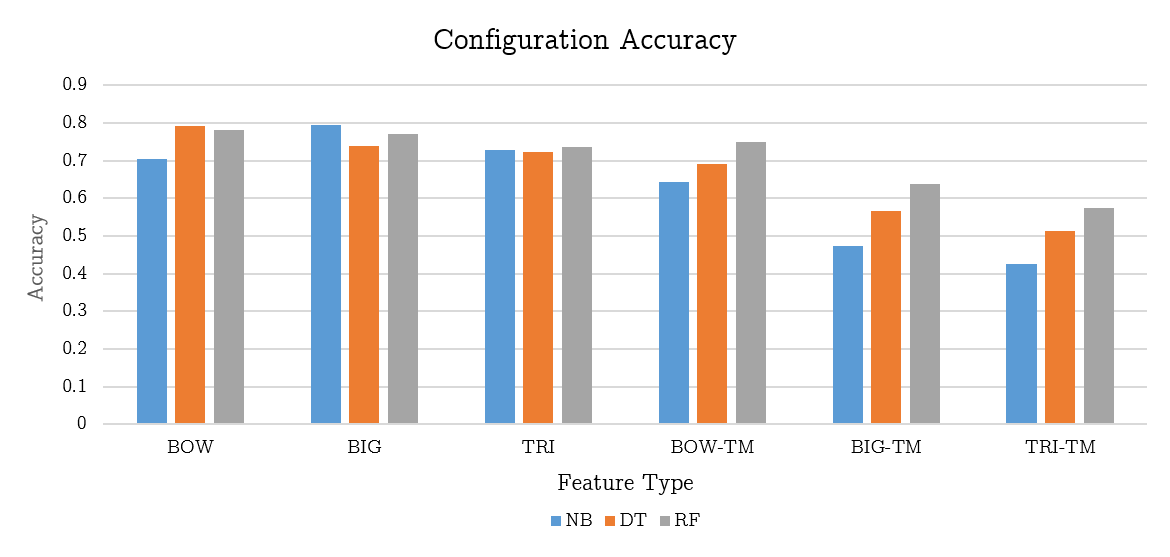
\includegraphics[scale=0.8]{chart}
\end{center}
\caption{Configuration accuracy over classifiers and feature sets}
\label{chart}
\end{figure}

When considering all feature sets, random forests appeared to perform slightly better than others – on bi- and trigram feature sets, it outperformed naïve Bayes and decision tree considerably. This is because it is an ensemble method and is designed to produce better results though using a number of slightly better-than-average classifiers. It seemed that on the weaker feature sets, random forests did particularly well. For example, it out-performed the other classifiers on all metrics for all topic models. 

In terms of the stronger feature sets of uni- and bigrams, the classifiers performed quite similarly. Na{\"i}ve Bayes did not perform as well as decision trees or random forests on unigrams, whereas it outperformed both for bigrams. This could be because bigrams offer the classifier a greater chance to condition its probabilities further, whereas the unigram approach is likely to see a much higher average term frequency with respect to a topic. Over all metrics, na{\"i}ve Bayes performed better than the other classifiers on bigrams by at least half a percentage point but more commonly by at least two percentage points. Considering how close the classifier performance is, this is a reasonable distance.

Decision trees and random forests performed quite similarly on unigrams. One would expect similar performance since random forests is effectively generating a range of decision trees to classify with. For all metrics, the performance was very close (if not effectively identical in some places). It can be seen here that the ensemble method is producing effectively the same result as the standalone tree, indicating that little is gained from the extra classifier training and result voting. This could be because, since the basic tree is sufficiently good already, having a range of good trees simply produces the same result. The singular decision tree was chosen as the optimal classifier since unigrams were chosen as the optimal feature and over this feature set, the classifier slightly outperformed random forests in terms of accuracy, whilst the other metrics were almost identical. With that in mind, using random forests would have been equally acceptable due to how close the performance was. 

\subsection{Optimal Classifier Performance}
In order to test the chosen configuration of classifier and feature set, the test data was used. Since some judgement of correctness was needed, the system was only tested on instances where topics were present and as when training the classifiers, multiple topics saw the article used once for each topic. In terms of testing, this will result in some guaranteed misclassifications for the classifier as it cannot, using a decision tree, offer two possible classifications for a given article. This is discussed below, but ultimately this was done at this stage to match the testing method to the training method in the interest of fairness. The results can be seen in Table~\ref{tab:opt}, and the relevant code can be seen in \texttt{run\_bag\_of\_words\_test} in \texttt{helper.py}.

% Table generated by Excel2LaTeX from sheet 'Sheet3'
\begin{table}[htbp]
  \centering
  \caption{Optimal Configuration Results}
    \begin{tabular}{rrrr}
    \toprule
    Accuracy & Recall & Precision & F-measure \\
    \midrule
    0.7976 & 0.7976 & 0.7957 & 0.7966 \\
    \bottomrule
    \end{tabular}%
  \label{tab:opt}%
\end{table}%


The accuracy, precision and recall of this configuration is quite good with all three being at 79\%. Whilst further tweaking and training might produce a higher accuracy, this is a good starting point. By adjusting the tree parameters or performing post-pruning, statistical gains could be made. The similarity of this average to that on the training data is encouraging as it indicates that the classifier and feature set chosen do not heavily overfit the training data. To get a better gauge of this, however, a larger test set would need to be used.

Another area that could be further investigated is the effects of the inclusion of the article multiple times if it has multiple topics. As mentioned previously, this could cause overfitting but in favour of proper topic representation. Instead, a better sample of training articles could be represented such that each has one topic and is sufficiently representative of this topic. Whilst this might raise performance, it may result in a higher chance of misclassification for ‘edge’ cases which could fit into multiple topics. As it stands, all classifier/feature set combinations effectively guarantee themselves some misclassifications since the classifiers will only produce a single label for a single article – predicting the article topic multiple times will simply produce the same label, thus giving at most one correct topic match.

\section{Clustering}
With the optimal classifier and feature set now chosen and tested, a range of clustering algorithms were used on the data. The methods used, from the SKLearn package, were:
\begin{itemize}
\item K-Means~\cite{kmeans}
\item DBSCAN~\cite{dbscan}
\item Ward's method~\cite{wards-meth}
\end{itemize}
Again, these were largely chosen to provide a range of classifiers over which to evaluate the performance. 

Ward's method is a hierarchical clustering method which is agglomerative, i.e. bottom up. It chooses clusters to merge via an optimal value of some objective function, specifically the minimum variance condition. This can be seen in Equation~\ref{ward-eq}. Ultimately this method was chosen as a baseline as at a high level, the Ward method provides quite a simple method of measuring distance between points. When dealing with a space of such high dimensionality as this project requires, this method may be somewhat limited. Regardless, as a baseline to the other methods, it can help discern if this task it well suited to clustering at all. In terms of implementation parameters, the main change from default was to set the number of clusters to find to be ten, to match the number of topics. The method \texttt{cluster\_ward} in \texttt{helper.py} implements this.

DBSCAN is a density based clustering method, in that it chooses clusters based on density distributions of nodes. It does this in a chain-like manner, traversing a series of nodes that are reachable from a randomly selected, unvisited one, adding each to the current cluster. In theory, this should relate reasonably well to topic prediction as each unigram configuration of articles relating to a given topic should occupy a relatively close space with respect to the vector space model. It also does not make assumptions about cluster shape, which is useful as the possible cluster shapes from the unigram feature set are not known. No non-default parameters were set for this algorithm. This can be seen in \texttt{cluster\_DB} in \texttt{helper.py}.

K-means groups instances into clusters by distance to cluster means – this is done by iteratively recalculating the cluster means and distances of points to them as more points are added to each cluster. The technique at its most fundamental is NP-hard, however heuristic methods are used to provide approximations – SKLearn uses Lloyd's algorithm~\cite{lloyds} to produce Voronoi cells in order to cluster. As with DBSCAN, this has the potential to classify articles reasonably well as it effectively attempts to identify the `perfect article' for a particular topic, then clusters articles based on distance to that topic. As with the Ward’s implementation, the only changed parameter from default was for the number of clusters – this was set to ten to match the number of topics. This is implemented in \texttt{cluster\_kmeans} in \texttt{helper.py}.

\subsection{Cluster Evaluation}
Each cluster was fitted in a similar way to the classifiers – the unigram representation of articles was provided (with an article represented multiple times if it had multiple topics), then was evaluated using the silhouette coefficient scoring metric. This is used when the expected clustering labels are unknown and evaluation is performed with the model itself. Although this system does have topic labels, it does not have cluster labels. These can differ since it is not necessarily known, especially methods such as DBSCAN which include an element of randomness, what these labels will be. Producing such labels would require, for example, manual running of the algorithm or some other pre-computing approach. The silhouette scores for each classifier can be seen in Table~\ref{tab:sil}.

% Table generated by Excel2LaTeX from sheet 'Sheet4'
\begin{table}[htbp]
  \centering
  \caption{Silhouette Coefficient Scores}
    \begin{tabular}{rrr}
    \toprule
    K-Means & DBSCAN & Ward's \\
    \midrule
    0.0663 & 0.0054 & 0.0603 \\
    \bottomrule
    \end{tabular}%
  \label{tab:sil}%
\end{table}%

Silhouette coefficients are between -1 and 1, with the former indicating that a sampled point would be better suited in a neighbouring cluster, and the latter indicating correct clustering. As seen in the results of the clustering, each method displays a coefficient of close to zero, with K-means and Wards displaying a value an order of magnitude higher than DBSCAN. This implies that all three of the clustering algorithms, on average, had an even split between correctly and incorrectly clustered instances. 


This could be due to a range of factors. Firstly, the dimensionality of the data might be too high for the clustering to be effective and make useful assumptions about the underlying distribution. This could be a result of not trimming the corpus back enough, though care would have to be taken in doing this to avoid oversimplifying the dataset. Another possible cause is the multiple-inclusion of articles. This effectively forces the clustering algorithms to try to cluster the same instance but in separate clusters, which will inevitably cause misclassification of some instances. 

\begin{equation}
\label{ward-eq}
d_{ij} = d(\{X_{i}\},\{X_{j}\}) = {\left\vert\left\vert X_{i} - X_{j} \right\vert\right\vert}^{2}
\end{equation}

% Table generated by Excel2LaTeX from sheet 'Sheet7'
\begin{table}[htbp]
  \centering
  \caption{Ward Clustering Assignments}
    \begin{tabular}{rr|r|r|r|r|r|r|r|r|r|r}
    \toprule
          &       & \multicolumn{10}{c}{Actual Topic Labels} \\
             &       & 1     & 2     & 3     & 4     & 5     & 6     & 7     & 8     & 9     & 10 \\
    \midrule \multicolumn{1}{c}{\multirow{10}[5]{*}{Cluster Labels}} & 1     & 162   & 91    & 322   & 28    & 42    & 119   & 233   & 18    & 7     & 11 \\
    \multicolumn{1}{c}{} & 2     & 788   & 0     & 0     & 1     & 0     & 0     & 0     & 1     & 0     & 0 \\
    \multicolumn{1}{c}{} & 3     & 650   & 0     & 0     & 0     & 0     & 0     & 0     & 0     & 0     & 0 \\
    \multicolumn{1}{c}{} & 4     & 234   & 458   & 0     & 1     & 3     & 0     & 0     & 0     & 1     & 0 \\
    \multicolumn{1}{c}{} & 5     & 5     & 17    & 32    & 219   & 282   & 205   & 2     & 145   & 95    & 98 \\
    \multicolumn{1}{c}{} & 6     & 443   & 0     & 0     & 0     & 0     & 0     & 0     & 0     & 0     & 0 \\
    \multicolumn{1}{c}{} & 7     & 0     & 0     & 0     & 122   & 1     & 7     & 0     & 12    & 79    & 46 \\
    \multicolumn{1}{c}{} & 8     & 302   & 64    & 0     & 17    & 9     & 1     & 2     & 1     & 13    & 4 \\
    \multicolumn{1}{c}{} & 9     & 125   & 858   & 9     & 7     & 14    & 5     & 5     & 15    & 3     & 2 \\
    \multicolumn{1}{c}{} & 10    & 0     & 0     & 98    & 0     & 0     & 0     & 47    & 0     & 0     & 0 \\
    \bottomrule
    \end{tabular}%
  \label{tab:ward}%
\end{table}%

% Table generated by Excel2LaTeX from sheet 'Sheet7'
\begin{table}[htbp]
  \centering
  \caption{DBSCAN Clustering Assignments}
    \begin{tabular}{rr|r|r|r|r|r|r|r|r|r|r}
    \toprule
          &       & \multicolumn{10}{c}{Actual Topic Labels} \\
          &       & 1     & 2     & 3     & 4     & 5     & 6     & 7     & 8     & 9     & 10 \\
    \midrule \multicolumn{1}{c}{\multirow{18}[10]{*}{Cluster Labels}} & 1     & 1181  & 0     & 0     & 0     & 0     & 0     & 0     & 0     & 0     & 0 \\
    \multicolumn{1}{c}{} & 2     & 330   & 0     & 0     & 0     & 0     & 0     & 0     & 0     & 0     & 0 \\
    \multicolumn{1}{c}{} & 3     & 0     & 0     & 39    & 0     & 0     & 0     & 22    & 0     & 0     & 0 \\
    \multicolumn{1}{c}{} & 4     & 0     & 0     & 17    & 0     & 0     & 0     & 6     & 0     & 0     & 0 \\
    \multicolumn{1}{c}{} & 5     & 0     & 0     & 0     & 2     & 2     & 3     & 0     & 0     & 2     & 0 \\
    \multicolumn{1}{c}{} & 6     & 0     & 0     & 0     & 2     & 0     & 0     & 0     & 0     & 2     & 2 \\
    \multicolumn{1}{c}{} & 7     & 5     & 0     & 0     & 0     & 0     & 0     & 0     & 0     & 0     & 0 \\
    \multicolumn{1}{c}{} & 8     & 0     & 0     & 0     & 2     & 0     & 0     & 0     & 0     & 1     & 2 \\
    \multicolumn{1}{c}{} & 9     & 0     & 0     & 10    & 0     & 0     & 0     & 11    & 0     & 0     & 0 \\
    \multicolumn{1}{c}{} & 10    & 0     & 0     & 0     & 3     & 0     & 0     & 0     & 0     & 3     & 0 \\
    \multicolumn{1}{c}{} & 11    & 0     & 0     & 2     & 0     & 0     & 0     & 4     & 0     & 0     & 0 \\
    \multicolumn{1}{c}{} & 12    & 0     & 0     & 0     & 5     & 0     & 0     & 0     & 5     & 0     & 0 \\
    \multicolumn{1}{c}{} & 13    & 0     & 0     & 2     & 0     & 0     & 2     & 2     & 0     & 0     & 0 \\
    \multicolumn{1}{c}{} & 14    & 6     & 0     & 0     & 0     & 0     & 0     & 0     & 0     & 0     & 0 \\
    \multicolumn{1}{c}{} & 15    & 0     & 0     & 0     & 3     & 0     & 0     & 0     & 0     & 3     & 3 \\
    \multicolumn{1}{c}{} & 16    & 0     & 0     & 4     & 0     & 0     & 0     & 3     & 0     & 0     & 0 \\
    \multicolumn{1}{c}{} & 17    & 0     & 0     & 0     & 0     & 0     & 0     & 6     & 0     & 0     & 0 \\
    \multicolumn{1}{c}{} & 18    & 0     & 0     & 0     & 2     & 0     & 0     & 0     & 0     & 2     & 2 \\
    \bottomrule
    \end{tabular}%
  \label{tab:hier}%
\end{table}%

% Table generated by Excel2LaTeX from sheet 'Sheet7'
\begin{table}[htbp]
  \centering
  \caption{K-Means Clustering Assignments}
    \begin{tabular}{rr|r|r|r|r|r|r|r|r|r|r}
    \toprule
          &       & \multicolumn{10}{c}{Actual Topic Labels} \\
            &       & 1     & 2     & 3     & 4     & 5     & 6     & 7     & 8     & 9     & 10 \\
    \midrule \multicolumn{1}{c}{\multirow{10}[5]{*}{Cluster Labels}} & 1     & 442   & 0     & 0     & 0     & 0     & 1     & 0     & 0     & 0     & 0 \\
    \multicolumn{1}{c}{} & 2     & 90    & 591   & 87    & 190   & 245   & 232   & 16    & 164   & 76    & 57 \\
    \multicolumn{1}{c}{} & 3     & 400   & 316   & 4     & 34    & 80    & 36    & 3     & 12    & 18    & 19 \\
    \multicolumn{1}{c}{} & 4     & 534   & 0     & 0     & 0     & 0     & 0     & 0     & 0     & 0     & 0 \\
    \multicolumn{1}{c}{} & 5     & 265   & 540   & 0     & 0     & 5     & 0     & 0     & 0     & 0     & 0 \\
    \multicolumn{1}{c}{} & 6     & 443   & 0     & 0     & 0     & 0     & 0     & 0     & 0     & 0     & 0 \\
    \multicolumn{1}{c}{} & 7     & 60    & 40    & 272   & 7     & 21    & 67    & 222   & 6     & 3     & 4 \\
    \multicolumn{1}{c}{} & 8     & 475   & 0     & 0     & 0     & 0     & 0     & 0     & 0     & 0     & 0 \\
    \multicolumn{1}{c}{} & 9     & 0     & 1     & 0     & 163   & 0     & 1     & 0     & 10    & 100   & 81 \\
    \multicolumn{1}{c}{} & 10    & 0     & 0     & 98    & 1     & 0     & 0     & 48    & 0     & 1     & 0 \\
    \bottomrule
    \end{tabular}%
  \label{tab:kmean}%
\end{table}%


In order to estimate accuracy with respect to original topic labels, an indirect approach had to be used. As, without pre-calculation, predicting cluster labels and mapping them to topic labels is not possible, the system instead attempts the count the number of actual topic labels in each cluster. It does this by finding the instances in each cluster, then gathering their topic labels and grouping these by their value. The \texttt{ run\_bag\_of\_words\_cluster} in \texttt{helper.py} implements this. The results can be seen in Tables~\ref{tab:ward},~\ref{tab:hier} and~\ref{tab:kmean}. Note that the topics are assigned as follows:
\begin{enumerate}
\item earn
\item acquisitions
\item money-fx
\item grain
\item crude
\item trade
\item interest
\item ship
\item wheat
\item corn
\end{enumerate}
Firstly, it is clear to see that DBSCAN performs poorly. It manages to classify a lot of the articles under topic 1 correctly but the vast majority of the articles are missing from the labelled set entirely. This is because DBSCAN labels anything it classes as noise with a -1, which in this case, were removed from the label comparison. As such, whilst it seemingly manages to classify earn-related topics well, it does very poorly otherwise. This could be due to the fact that the instance space is likely to be very dense due to the reuse of articles for a variety of topics, so DBSCAN would prefer one large cluster to many smaller ones. This is furthered by the fact that DBSCAN assumes clusters are formed of dense regions surrounded by sparse areas.

K-means performed more effectively, managing to allocate some clusters to articles predominately from one class, for example cluster label 1 maps well to topic 1. It does seem to suffer from partitioning the instances of the same class, as cluster label 6 also sees a high number of topic 1 articles. Cluster labels 2, 3 and 7 display a wider spread of topics, with 2 having a clear majority of topic 2 articles. Whilst this is better, it is not at all close to the decision tree classifier. There is still a lack of clusters with a clear majority of a single topic and a number of splits between cluster labels, especially on topic 1. Ward clustering encountered the same issues as K-means, with some clusters containing a majority of one topic, and some with a spread across many. As with DBSCAN, it seems that the density of the instance space, coupled with the fact that two articles of different topics may contain a number of similar words, makes the clustering somewhat inaccurate.

In general, clustering does not seem effective on a dataset such as this. Largely, this seems to be due to the density of the instance space, making it very difficult to partition into clusters. This not only causes articles of the same topic to be split into separate clusters, but also makes the success of the clustering algorithm heavily depend on any random elements involved – the choice of points to begin clustering at will make a large difference.  


\section{Conclusion}
This project has produced a system through which articles from the Reuters dataset can be classified based on topic. Through using a combination of pre-processing, unigram representation and decision tree classification, the system has almost an 80\% accuracy rate over tested articles. Whilst clustering was tested as an alternative to supervised learning, it did not perform as well, instead giving average performance across all three algorithms used. As such, with further tuning and training, the unigram and decision tree combination seems to have further potential in classification of such articles.

\bibliography{biblio}
\bibliographystyle{plain}

\end{document}